\documentclass{article}
\usepackage[utf8]{inputenc}
\usepackage{xcolor}

\usepackage{tikz}
\usetikzlibrary{shapes.geometric, arrows}

\tikzstyle{startstop} = [rectangle, rounded corners, minimum width=3cm, minimum height=1cm,text centered, draw=black, fill=red!40]
\tikzstyle{io} = [trapezium, trapezium left angle=70, trapezium right angle=110, minimum width=3cm, minimum height=1cm, text centered, draw=black, fill=blue!30]
\tikzstyle{process} = [rectangle, minimum width=3cm, minimum height=1cm, text centered, draw=black, fill=orange!60]
\tikzstyle{decision} = [diamond, minimum width=3cm, minimum height=1cm, text centered, draw=black, fill=green!30]
\tikzstyle{arrow} = [thick,->,>=stealth]


\title{Financial Bootcamp}
\author{Liza Dahiya}
\date{May 2020}
\begin{document}

% \pagecolor{black}
% \color{white}

\maketitle
\tableofcontents
\section{Various Financial statements}
\begin{itemize}
    \item Profit \& loss statement (Income and Expenses)
    \item Cash Flow statement (Inflow and Outflow)
    \item Balance Sheet (Liabilities and Assets)
\end{itemize}
\textbf{Example:} \par
Company sells 100 cars for 10 lakhs and cost for manufacturing them was 8 lakhs in a financial year. So the the Profit and loss statement records the \textit{\textbf{business transactions}} to be 100*2 lakhs which is 2 crore. Now lets say that 50 cars were sold to government of India which promised to pay after an year. Hence in this case the total inflow was 50*10 lakhs while the outflow was 100*8 lakhs which means that the \textbf{\textit{cash transactions}} is negative, which is recorded on the cash-flow statement. 
\subsection{Balance Sheet}
It looks at what you owe i.e. liabilities and what you own i.e. assets. Sources of fund include share capital/equity and debt i.e. liabilities and application of these funds include long term tangible and non-tangible assets, investments and short term assets. At any given point of time, liabilities must balance out assets.
\par It is cumulative, additive and it keeps on adding the previous year data.
\par Net worth of the company is the total liabilities owed by a company. 
\subsection{Profit and Loss Statement}
Profit measures a company's well-being and it is also termed as income statement. It is measured over a certain period of time. \par
Attributes of P\&L statements:
\begin{itemize}
    \item Sales
    \item Cost of goods sold: raw material, direct labour, direct electricity
    \item Subtracting COGS from sales, we get the gross profit
    \item Other operating expenses: marketing, employees salaries
    \item Subtracting these expenses from Gross Profit we get: Earnings Before Interest, Tax, Depreciation and Amortization. \textbf{(EBITDA)}i.e. operating profit 
    \item Subtracting depriciation and amortization from EBITDA, we're left with \textbf{EBIT}
    \item After subtracting tax1es and interests, we've the \textbf{Net Profit}.
\end{itemize}
\subsection{Cash Flow Statement}
Profitable yet cash strained: when the payment is to be made after an year, for say. Technically if the company is negative cash valued then profitability is of no use.
\begin{enumerate}
    \item Operating Activities
    \item Investments Activities
    \item Financial Activities
\end{enumerate}
\subsubsection{Indirect Method of cash flow creation:}
Start with \textbf{Net Profit} of a company, is the cash inflow of the company. Then we add \textbf{depreciation}. Then add \textbf{Non-Cash costs} i.e. accounting the depreciation and amortization and then subtract the \textbf{capital expenditure}. Then we look at receivable which means that the sales have been made but the payment has not yet been received, this \textbf{change in receivable} amount is subtracted since it was added in the sales term while counting the net profit. Then we look at the payable which is the money still available with us and it had earlier been subtracted in the cost section but we realize that the payment has not yet been done. Hence we add change in \textbf{current liabilities} and subtract change in \textbf{current assets}, We also add \textbf{change in debt} and subtract \textbf{dividend}, which is the amount paid to the shareholders and this finally gives us \textbf{cash flow}.  


\section{Indian Financial System}
\subsection{Need of Financial System}
\begin{itemize}
    \item Access to Capital: Fuel Growth
    \item Management of Capital: Manage Risk 
\end{itemize}
\subsection{Components of Financial System}
\begin{itemize}
    \item \textbf{Institutions}: RBI, SEBI, and other players; who regulate rules and ensure proper functioning of financial system and other players include banks.
    \item \textbf{Markets:} Equity (raise money through shares) and Debt Markets (raise money through loans); Equity Market in India include NSE/BSE, while Debt Market isn't that popular in India.
    \item \textbf{Instruments:} Debt and Equity or hybrid 
\end{itemize}
\subsubsection{Financial Institutions}
\begin{enumerate}
    \item \textbf{RBI}
    \begin{itemize}
        \item Maintain value of Currency
        \item Maintain Liquidity: Monetary Policy
        \item Control Inflation
        \item Promote New initiatives
        \item And watch economic progress
    \end{itemize}
    
    \item \textbf{SEBI} \par
    Take Market related decisions.
    \begin{itemize}
        \item Provide a good environment for issuers
        \item Protect investors and their rights
        \item Regulate intermediates 
        \item Regulate Financial Market entities i.e. mutual funds 
    \end{itemize}

    \item \textbf{Bank}
    \begin{itemize}
        \item Idea is to provide capital
        \item While managing risks
    \end{itemize}
    
    \item \textbf{Others financial institutions}\par
    NBFC (Non-Banking Financial Company), Brokers, Credit rating agencies, Leasing agencies, Exchanges, Assets and Management companies i.e. Mutual Funds, Grush finance, etc.
\end{enumerate}

\subsubsection{Financial Markets}
The financial markets in India could be classified in three ways as follows:
\\
\begin{enumerate}
     
\item Stocks/ shares trade on stock/ equity market and debentures or bonds trade in Debt Market.

\begin{center}
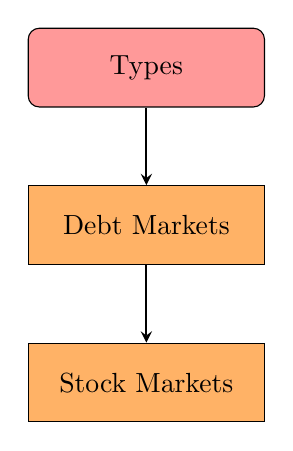
\begin{tikzpicture}[node distance=2cm]
\node (start) [startstop] {Types};
\node (pro1) [process, below of=start] {Debt Markets};
\node (pro2) [process, below of=pro1] {Stock Markets};
\draw [arrow] (start) -- (pro1);
\draw [arrow] (pro1) -- (pro2);
\end{tikzpicture}
\end{center}

\item When IPO or sharing of securities is done for the first time it is called primary market, after initial securities are traded off then any further trading comes under the secondary markets.

\begin{center}
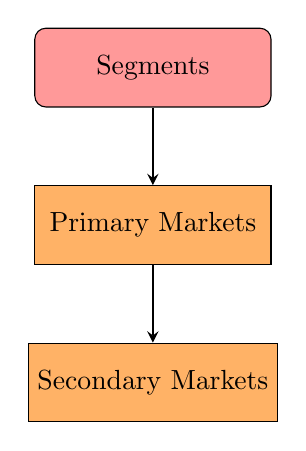
\begin{tikzpicture}[node distance=2cm]
\node (start) [startstop] {Segments};
\node (pro1) [process, below of=start] {Primary Markets};
\node (pro2) [process, below of=pro1] {Secondary Markets};
\draw [arrow] (start) -- (pro1);
\draw [arrow] (pro1) -- (pro2);
\end{tikzpicture}
\end{center}


\item Organised markets include Banks and NBFC Exchange and unoragnised include Peer-to-Peer lending, P2P and direct loan

\begin{center}
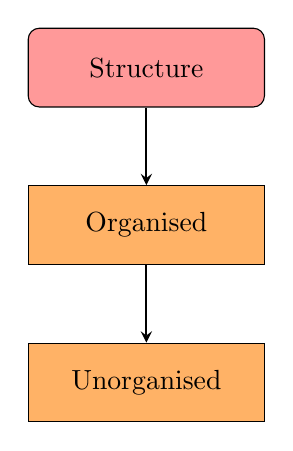
\begin{tikzpicture}[node distance=2cm]
\node (start) [startstop] {Structure};
\node (pro1) [process, below of=start] {Organised};
\node (pro2) [process, below of=pro1] {Unorganised};
\draw [arrow] (start) -- (pro1);
\draw [arrow] (pro1) -- (pro2);
\end{tikzpicture}
\end{center}
\end{enumerate}
\section{Financial Markets}
There are two types of Indian stock markets: National stock Exchange, NSE and Bombay Stock Exchange, BSE.\par
A stock market essentially allows the flow of capital in the economy from the people who are saving to the people/company who are in need of the money. If one buys can \textbf{equity} in a company, (s)he becomes a shareholder and have a share in the profit of the company, whereas if (s)he buys \textbf{bonds}, they become debt holder and have a fixed income. For such exchanges, one needs a \textbf{broker} who is listed on the stock exchange. 
\begin{center}
    Market Cap = Total shares of the company* Market price
\end{center}
Broadly, market cap is the amount of money that will be required to purchase the entire company.
\begin{center}
    Market Cap Free Float = Total MCap- Promoters share
\end{center}
Promoters share are the shares owned by the owner of the company. 
\section{Industry Analysis}
The term \textbf{economic moat}, popularized by Warren Buffett, refers to a business' ability to maintain competitive advantages over its competitors in order to protect its long-term profits and market share from competing firms.
\subsection{Porter 5 forces}
\begin{enumerate}
    \item \textbf{Intensity of competitive rivalry} \par
    Very high competitive rivalry leads to \textbf{price wars}, which lead to profits margin reduction for most of the companies. \textbf{Ex:} Airlines, commerce and telecom.  
    \item \textbf{Threats of new entrants} \par
    This is basically governed by: regulations, capital intensity of market, brand/reach of companies. \textbf{Ex:} Soap companies like Lifeboy and Lux enjoy low threats from entrants because of their brand value while telecom/airlines have low such threats because of government regulations. 
    \item \textbf{Threats of substitute products} \par
    This includes threats from the advancing technology. \textbf{Ex:} Reliance faced threats from the shifts towards cleaner fuel and hence expanded its business from existing oil to retail and telecom. 
    \item \textbf{Bargaining Power of Suppliers} \par
    If this is high, then there is pressure on input rates and very low payable cycle. 
    \item \textbf{Bargaining Power of Buyers} \par
    If the business is B2B then this bargaining power will be high as compared to when it is B2C. 
\end{enumerate}
\subsection{Factors that affect valuation}
\begin{enumerate}
    \item \textbf{Competitive advantage} \par
    Brand, Government Regulation, Distribution Network, Operational Efficiency, Gestation Period, Low Supplier Bargaining Power, No ready substitute product, cost competitiveness, Low Customer Bargaining Power, Supply side economies of sale, Demand side economies of sale 
    \item \textbf{Growth}
    \item \textbf{Opportunity Size}
    Analysis of growth rate. \textbf{Ex:} Hospital beds market in India. And penetration of the market also plays a role. 
    \item \textbf{Stability}
    \textbf{Ex:} Steel market has more volatile as compared to FMGC companies. 
\end{enumerate}

\section{Capital Budgeting}
\subsection{The Concept of Present Value}
It is obvious that the value of ccash today will be much lesser than that after lets say n years. So to find the present value, $PV$; we need to see how much is the cash flow $CF$; and at which year $n$ are we calculating the value. We take the rate of interest to be $r$, which is defined by the risk. 
$$PV = \frac{CF_n}{(1+r)^n}$$
\subsubsection{Net Present value}
It is the present value of cash inflows minus the present value of the cash outflow.\par
If, $NPV>0$ then, value is being created else value is destroyed.

\subsection{Internal Rate of Return}
It is the rate at which NPV of a project turns zero. At rates higher than IRR, the project will not be feasible. Simply put, IRR is the maximum rate that can come out of a project. Any rate higher than IRR will turn NPV negative. 
\subsection{Application of NPV}
\begin{itemize}
    \item Valuation of Stock
    \item Valuation of Bonds
    \item Calculation of EMIs
    \item Derivative Pricing
\end{itemize}

\section{Return Calculations}
\subsection{Average Return}
While calculating average return we need to look at the geometric mean.
$$(1+r_{avg})^2 = (1+r_1)(1+r_2)$$
\subsection{The Concept of CAGR}
Compound annual growth rate is a business and investing specific term for the geometric progression ratio that provides a constant rate of return over the time period.
$$CAGR = (\frac{Final}{Initial })^{\frac{1}{n}}-1$$

\section{Ratio Analysis and Interpretations}
Ratios are the number that are used to quantitative data which we find in a company's financial statement. It is derived by dividing one data point by another. It can be used to compare:
\begin{itemize}
    \item with other industrial players
    \item historical performance of company
    \item with budget or target.
\end{itemize}
They tell us about the financial health of a company. 
\subsection{Ratio Types}
\begin{enumerate}
    \item \textbf{Profitability Ratio}
    \begin{itemize}
        \item \textbf{Operating Profits Margin}: Operating Profit (EBITDA/EBIT) /Sales 
        \item \textbf{Net Profit Margins}: Net Profit/Sales
    \end{itemize}
    \item \textbf{Return Ratio}
    \begin{itemize}
        \item \textbf{Return on Capital Employed}: EBIT/ (Shareholder Funds + Funds) or 
        EBIT (1-t)/Total Assests
        \item \textbf{Return on Net Worth}: Net Profit/(Share capital + reserves)
    \end{itemize}
    \item \textbf{Coverage Ratio}\\
    A \textbf{coverage ratio}, broadly, is a group of measures of a company's ability to service its debt and meet its financial obligations such as interests payments or dividends.
    \begin{itemize}
        \item \textbf{Interest covreage ratio}= EBIT/Interest
    \end{itemize}
    A coverage ratio \textbf{below 1} indicates a company cannot meet its current interest payment obligations and, therefore, is not in good financial health.
    \item \textbf{Stability Ratio}
    \begin{itemize}
        \item \textbf{Debt/Equity}= Long term Debt/ Equity
    \end{itemize}
    \item \textbf{Liquidity Ratio}
    \begin{itemize}
        \item \textbf{Current Ratio:} Current Assets/Current Liabilities
        \item \textbf{Quick Ratio:} (Cash+Receivables)/Current Liabilities
    \end{itemize}
    \item \textbf{Turnover Ratios}
    \begin{itemize}
        \item \textbf{Inventory Turnover Ratio}: Sales/Inventory
        \item \textbf{Receivable Turnover Ratio}: Sales/Receivables
        \item \textbf{Assets Turnover Ratio}: Sales/Total Assets
        \item \textbf{Fixed Asset Turnover Ratio}: Sales/Fixed Asset
    \end{itemize}
\end{enumerate}
\subsection{DuPont-Analysis}
\begin{itemize}
    \item \textbf{Net Profit Margin}: Net Profit / Net Sales\\
    An increase in this would show increase in profitability.
    \item \textbf{Total Asset Turnover Ratio}: Sales / TA\\
    An increase here would show better efficiency
    \item \textbf{Leverage} \textbf{Factor}: Total Assets / Equity\\
    An increase here would show an increase in asset with respect to the equity. 
    \end{itemize}
    ROE is calculate by the multiplication of the three terms. i.e. \\
    \textbf{ROE} = Net Profit Margin $*$ Total Asset Turnover Ratio $*$ Leverage Factor.
\end{document}
